\newpage
\section{Diskussion}
\label{sec:diskussion}
Beginnend mit den Temperaturprofilen der Wärmetauscher für die Reihen- und Parallelschaltung werden an dieser Stelle die Messergebnisse diskutiert und bewertet. Die in der Abbildung \ref{dia:temp_profil} dargestellten Temperaturverläufe, welche über den Rohrabschnitt aufgetragen wurden,  geben erste Indizien zur Bewertung der beiden Fahrweisen. Es zeigt sich, dass die Temperaturverläufe für den parallelen Betrieb deutlich steiler zu laufen als für die Reihenschaltung. Zu erkennen ist ebenfalls, dass die Temperaturdifferenzen der Parallelschaltung größer sind, als die der Reihenschaltung. Somit lässt sich die Vermutung aufstellen, dass die Parallelschaltung die effizientere Wärmeübertragung für die jeweils eingestellten Volumina liefert. Jedoch sollte beachtet werden, dass für beide Verfahren unterschiedliche Volumenströme gefahren werden. Somit kann anhand dieses Diagramm lediglich die Fahrweisen mit den entsprechenden Betriebsparametern verglichen werden, geben jedoch keine Auskunft über den Vergleich von Reihen- und Parallelschaltung.\\

Anhand der Wärmeströme lassen sich nun beide Fahrweisen quantitativ in Form von Wärmeströme unterscheiden. Die Korrektur der Volumenströme ist hierbei notwendig und gibt Auskunft über den Fehler der Messungen am jeweiligen System. Auch an dieser Stelle der Auswertung wird deutlich, dass der Parallelbetrieb Vorteile in Bezug  wird deutlich, dass die Menge an übertragener Wärme höher ist als bei der Reihenschaltung. Es würde sich demnach auch hier wieder auf eine höhere Effizienz des Parallelbetriebs schließen lassen.\\

Zieht man in die Betrachtung nun auch die Wirtschaftlichkeit der jeweiligen Fahrweise mit ein, so setzt man die übertragene Wärmemenge in ein Verhältnis zur benötigen elektrischen Leistung für die Förderung des Fluides. Wirtschaftlichkeit bedeutet in diesem Fall, dass maximal viel Wärme übertragen wird, für eine minimale, elektrische Leistung der Pumpe. Demnach ist das Ziel möglichst hohe Werte für dieses Verhältnis zu erreichen. Es zeigt sich, dass die Werte für die Parallelschaltung deutlich wirtschaftlicher erscheinen als die Reihenschaltung, aufgrund der höheren Menge an übertragenen Wärme über den auszugleichenden Druckverlust. Auch unter diesem Aspekt besticht die Parallelschaltung als Fahrweise in diesem Versuchsaufbau.

\begin{figure}[h!]
	\begin{center}
		\resizebox{0.8\textwidth}{!}{
			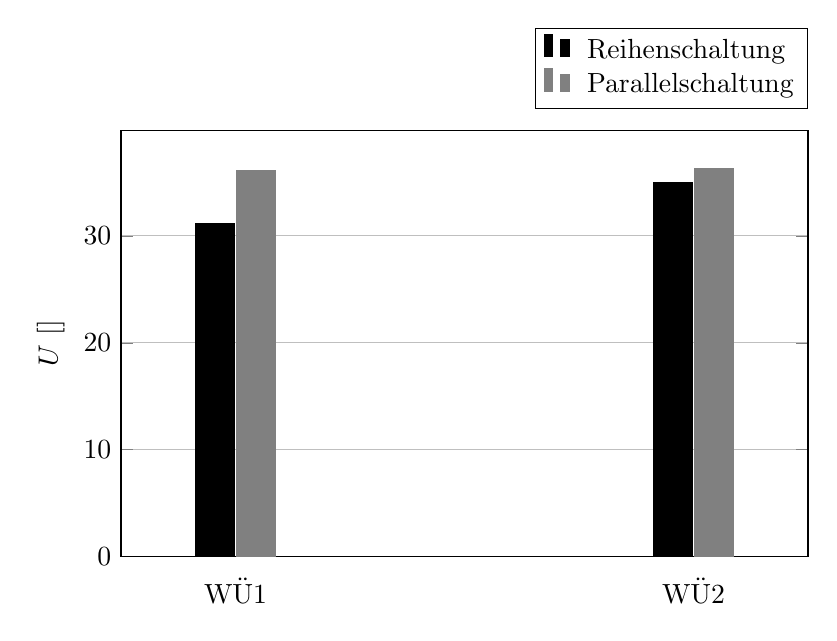
\begin{tikzpicture}
			\begin{axis}[
			width  = 0.85*\textwidth,
			height = 7cm,
			major x tick style = transparent,
			ybar=2*\pgflinewidth,
			bar width=14pt,
			ymajorgrids = true,
			ylabel = {$U \, \left[\si{\watt \per \meter\per\kelvin}\right]$},
			symbolic x coords={WÜ1,WÜ2},
			xtick = data,
			scaled y ticks = false,
			enlarge x limits=0.25,
			ymin=0,
			legend cell align=left,
			legend style={
				at={(1,1.05)},
				anchor=south east,
				column sep=1ex
			}
			]
			%Reihenschaltung
			\addplot[style={black,fill=black,mark=none}]
			coordinates {(WÜ1, 31.13) (WÜ2,34.98)};
			
			%Paralaleschaltung
			\addplot[style={gray,fill=gray,mark=none}]
			coordinates {(WÜ1,36.13) (WÜ2,36.27)};
			
			
			\legend{Reihenschaltung, Parallelschaltung}
			\end{axis}
			\end{tikzpicture}
		}
		\caption{Grafischer Vergleich der Wärmedurchgangskoeffizienten}
		\label{dia:durchng}
	\end{center}
\end{figure}
\FloatBarrier

